%% The first command in your LaTeX source must be the \documentclass command.
%%
%% Options:
%% twocolumn : Two column layout.
%% hf: enable header and footer.
\documentclass[
% twocolumn,
% hf,
]{ceurart}

%%
%% One can fix some overfulls
\sloppy

%%
%% Minted listings support 
%% Need pygment <http://pygments.org/> <http://pypi.python.org/pypi/Pygments>
\usepackage{listings}
%% auto break lines
\lstset{breaklines=true}

\usepackage{svg}
\usepackage{graphicx}
\usepackage{sepfootnotes}

\newcommand{\rt}[1]{\noindent\textcolor{red}{{\bf \{RT}: #1{\bf \}}}}

%%
%% end of the preamble, start of the body of the document source.
\begin{document}

%%
%% Rights management information.
%% CC-BY is default license.
\copyrightyear{2024}
\copyrightclause{Copyright for this paper by its authors.
  Use permitted under Creative Commons License Attribution 4.0
  International (CC BY 4.0).}

%%
%% This command is for the conference information
\conference{Alberto Mendelzon International Workshop on Foundations of Data Management}

%%
%% The "title" command
\title{Opportunities for Shape-based Optimization of Link Traversal Queries over Decentralized Environments}


%%
%% The "author" command and its associated commands are used to define
%% the authors and their affiliations.
\author[1]{Bryan-Elliott Tam}[%
]

\author[1]{Ruben Taelman}[%
]
\author[1]{Pieter Colpaert}[%
]


\address[1]{IDLab,
Department of Electronics and Information Systems, Ghent University – imec}

%%
%% Keywords. The author(s) should pick words that accurately describe
%% the work being presented. Separate the keywords with commas.
\begin{keywords}
  Linked data \sep
  Link Traversal Query Processing \sep
  Query containment \sep
  RDF shape \sep
  Descentralized environments
\end{keywords}

%%
%% This command processes the author and affiliation and title
%% information and builds the first part of the formatted document.
\maketitle


\rv{In the title, shall we remove \enquote{over Decentralized Environments}? That's a given.}

\begin{abstract}
    % Context
    ~\rv{The next sentence is not relevant context for our target audience. Let's remove.}
    \remove{
    Linked Data on the Web can be considered as one very large Decentralized Knowledge Graph.
    }
    While centralized query processing approaches are well-understood,
    decentralization-friendly alternatives with no prior indexing such as Link Traversal Query Processing (LTQP)
    are insufficiently performant for real-world use cases.
    LTQP approaches on the web are difficult due to the pseudo-infinite size of the domain,
    the unstructured nature of the medium,
    and the lack of a priori information for query planning.
    For most traversal-based queries the execution of a large number of HTTP requests is the bottleneck. 
    However, in practice, queries target small subsets of the Web.
    Web subsets are always structured either implicitly or explicitly.
    Explicit structure can be described via hypermedia descriptions.
    Query engines can improve their performance by using structural information to reduce their search domain.
    \rv{So I've come to this point, but I have not read an actual need or a~problem. It's all context. WHY do we need LTQP? What do you want to do? What do you want to achieve? I think you might want to tell me the following. \textbf{CONTEXT:} hey, a lot of data is spread across many different places---and we cannot bring it together first, because of legal reasons (licenses, personal data laws, \ldots). Although decentralized query is thus a necessity, it's too slow.}
    % Need
    \rv{\textbf{NEED:} Figuring out to what extent shapes help us get speed back.}
    % Task
    \rv{Try to phrase the next more strongly, as a task you have done (past tense), not what this paper does (that's the Object bit later). We didn't just explore; we did something really specific. Please tell us that thing here.}
    In this paper, we explore the opportunities of using mappings between RDF data shapes and distributed RDF subgraphs
    for the purpose of improving the performance of traversal-based queries.
    % Object
    \rv{I think we can be more specific here (this sentence applies to every paper in the world.)}
    In this article, we discuss these opportunities, present preliminary results, and discuss potential future work.
    % Findings
    Our initial experiments show that with little maintenance and work from the server,
    our method can significantly reduce the number of links traversed to answer a query leading to
    a substantial reduction in query execution time compared to the state of the art.
    \rv{Great; are there specific numbers we can mention in the previous sentence?}
    % Perspectives
    \rv{This is not a place for promises about what we will do. It's a place to show how others can build upon our work. (And we might be those others, but that's not relevant.)}
    In future work, we will formalize our method, perform more extensive experiments,
    and design algorithms for query planning that take this shape metadata into consideration.
\end{abstract}

\section{Introduction}
 
The large-scale publication of linked data empowers more freedom in the creation and usage of web applications.
More concretely linked data can diminish data silos \cite{Verstraete2022}
and could foster potential new forms of application ownership \cite{Mechant2021}.
The \href{https://solidproject.org/TR/protocol}{Solid} and
\href{https://docs.joinmastodon.org/}{Mastodon} protocols
are popular technologies utilizing the emancipatory potential of linked data.
Linked data is mostly modeled and published using the graph data formalization \href{https://www.w3.org/TR/rdf12-concepts/}{RDF} and its serializations.
RDF terms can be expressed using IRIs, Blank Nodes, and Litterals.
The usage of IRIs provides more reusability of data and explicitizes in a machine-interpretable way the relations between
information from multiple remote or local subgraphs.
More information about an IRI term can be found if it is dereferenceable (treated as a URL) using the HTTP protocol.


The web is a decentralized wealth of information.
Index servers and the query language webSQL \cite{Mendelzon1996} propose a mechanism to capture this knowledge using conjunctive queries.
However, this approach relies on prior indexing, which can be restrictive and hinder the natural serendipity of the web. 
Link Traversal Query Processing (LTQP) \cite{Hartig2012} propose to replace the index servers with descriptive dereferenceable IRIs 
preserving the natural link between information in the web.
LTQP starts with a few URIs called seed URIs and recursively dereferences them from an internal data source following a lookup policy.
While LTQP enables live exploration of environments without prior indexing, it leads to some difficulties.
One of them is the pseudo-infinite search domain derived from the size of the World Wide Web \cite{hartig2016walking}.
Additionally, HTTP requests can be very slow and unpredictable making their execution the bottleneck of the method \cite{hartig2016walking}.
Reachability criteria \cite{Hartig2012} are a partial answer to this problem by defining completeness on the traversal of URIs
contained in the internal data source of the engine instead of on the acquisition of all the results or the traversal of the whole web.
Those criteria can also be used as a lookup policy for dereferencing of external data sources.
Another difficulty is the lack of a priori information about the sources rendering query planning arduous.
To alleviate this problem, the current state of the art consists of using carefully crafted heuristics for joins ordering \cite{Hartig2011}.
Those heuristics provide non-optimal fairly performant query plans.
The limitations of this approach are usually of little importance because the main bottleneck is the high number of HTTP requests.
In response to this, current research focuses on providing fast results to the user by ordering adequately the dereferencing operations of IRIs \cite{hartig2016walking}.

Previous LTQP research didn't consider the particular structure of the querying environment.
Environments like Solid described structures using more or less detailed hypermedia descriptions \cite{Fielding}.
We refer to the structures exploitable for query optimizations as structural assumptions.
Structural assumptions act as contracts between the data provider and 
the query engines stipulating that in a certain subdomain of the web, some information respecting a constraint can be found.
The approach consists of guiding the query engine towards relevant data sources by using 
those assumptions to discover and prune data \cite{verborgh2020guided}.
The usage of structural assumptions has been studied in Solid \cite{Taelman2023}.
The approach involves the utilization of the 
\href{https://solidproject.org/TR/protocol#resources}{solid storages} (that we refer to as Solid pods \cite{Taelman2023}) hypermedia description
to locate all the resources of a pod. 
This hypermedia description is derived from the \href{https://www.w3.org/TR/ldp/}{LDP specification}
which only captures the structures of storage but not their contents.
In response, the \href{https://solid.github.io/type-indexes/}{type index specification} is additionally used.
The type index propose a more declarative approach \cite{Taelman2017} by mapping RDF classes with sets of resources to perform dynamic optimizations.
It has been shown that by making query engines exploit those assumptions it is possible to reduce the query execution time
of realistic queries to the extent where the bottleneck is not the execution of 
HTTP requests but the suboptimal heuristic-based query plan \cite{eschauzier_quweda_2023, Taelman2023}.
Yet for multiple queries, the bottleneck remains the high number of HTTP requests  \cite{eschauzier_quweda_2023}.
It is reasonable to hypothesize that a significant portion of those HTTP requests lead to the dereferencing of
documents containing data that don't contribute to the result of the query.
Hence investigating more descriptive structural assumptions is a relevant research endeavor.

In this article, we propose to use RDF data shapes as the main mechanism for a structural assumption in the form of a Shape Index (SI).
The shape index is inspired by the type index.
However, it intend to be more expressive by describing the content of the data instead of only its class \cite{Taelman2017}.
% We could have used here as a reference the paper from Ben Demeester RDF Graph Validation Using Rule-Based Reasoning 
RDF data shapes are mostly used in data validation \cite{Gayo2018a} hence they provide an excellent means to describe data.
Yet to a lesser extent, they have been used in the context of federated query optimizations \cite{kashif2021}.
%RDF data shapes don't require significative power to be maintained because they only need to be edited 
%when the data model is modified.
%The low cost of maintenance combined with the mostly passive contribution of 
%the server when using RDF data shape for query optimization makes it a promising potential medium. 
We foresee opportunities for using a shape index during data source discovery, link pruning and ordering, and query planning.
This short paper presents our preliminary work on data discovery and link pruning.
\section{Shape index and query-shape containment}

\sepfootnotecontent{shapetrees}{
    \href{https://shapetrees.org/TR/specification/}{https://shapetrees.org/TR/specification/}
}

\sepfootnotecontent{fn:solidPrivacy}{
In this work, we do not take into consideration confidentiality restrictions.
}

\sepfootnotecontent{fn:litShapeComparaison}{
There exist comparisons between the shape and class definition approaches in the context of data validation~\cite{demeester_swj_2021} but it is left to be determined if their frame of comparison is compatible with our current problem
and foreseen opportunities.
}

The RDF specification does not enforce schemas on data.
However, the data published often adhere to an implicit schema due to the nature of the data and the formulation of RDF~\cite{Neumann2011CharacteristicSA}.
Implicit schemas have been used for query optimisation~\cite{Neumann2011CharacteristicSA, Meimaris2018HierarchicalCS}.
We propose to adapt those methods for LTQP by using explicit data schemas provided by the data provider in our source selection process.

The goal of the shape index is to reduce the query execution time by minimizing the dereferencing of unnecessary RDF documents in subdomains of the web (set of URL or URL patterns).
We define a shape index as a set of mappings between RDF data shapes and sets of resources.
This mapping concept shares similarities with shape mapping~\cite{Gayo2018} and target declarations~\cite{Gayo2018Shacl}.
However, instead of mapping shapes to RDF subgraphs, it maps shapes to documents.
It also shares some commonalities with \href{https://shapetrees.org/}{shape trees}~\sepfootnote{shapetrees}, however, it is designed to be a simpler formulation focused on query optimization.
To indicate the range of applications of the index an associated domain and a flag indicating if the shape index is \emph{complete} are defined.
A shape index is complete when every resource in the domain is associated with a shape within the shape index.
In a shape index when a shape is mapped to a set of RDF resources then the shape \emph{must} validate those resources.
Furthermore, every set of triples respecting the shape in the domain \emph{must} be located inside one resource of the set.

In order to determine before the traversal of a whole domain which resources are useful and which can be pruned in a defined subdomain, the query engine solves a \emph{query-shape containment} problem over the shape of the index similar to the classic query containment problem~\cite{afariQCE, Spasi2023, Chekol2018}.
The query containment problem consists of determining if the results of a query are a subset of the results of another query.
We propose to transform RDF data shapes into queries ($Q_{s}$)~\cite{labragayo2017validating, Corman2019, Delva2021} and apply similar resolution methods to query containment problems.
Due to the explicit domain definition of the index, this approach is adaptative, 
thus, the query engine can start its processing with permissive reachability criteria
such as $c_{all}$~\cite{Hartig2012} or the Solid state-of-the-art reachability criteria~\cite{Taelman2023}
and not suffer from the associated longer execution time during the traversal of environments containing a shape index.
The source selection process is schematized for a single domain in Figure~\ref{fig:shape_index}.
The process starts with the discovery of the shape index in the current (sub)domain.
In the case of Solid, the index can be at the root of the pod to be easily discoverable~\sepfootnote{fn:solidPrivacy}.
After the dereferencing of the index, the analysis is started inside the query engine.
The analysis consists of interpreting the binding results of the \emph{query-shape containment} problem.
The algorithm divides the query from the user into multiple star patterns with their dependencies ($Q_{star}$).
After the division of the query, the queries are pushdown~\cite{Stuckenschmidt2004, Yang2021FlexPushdownDBHP} to the level of source selection to evaluate if the $Q_{star}$ are contained inside the $Q_s$ of the shape index.
If all the $Q_{star}$ are contained in a $Q_{s}$ or have no binding with any $Q_{s}$
the reachability criterion is adapted to ignore all the resources not linked to a $Q_{s}$ even if the shape index is \emph{incomplete}.
If the shape index is \emph{complete} and not all the $Q_{star}$ are contained in a $Q_{s}$ the reachability criterion can be adapted
to visit every resource in relation to a $Q_{s}$ with a partial binding with a $Q_{star}$.
In a similar case with an \emph{incomplete} shape index, the query engine can only use the shape index for data discovery.
This case is similar to the usage of the type index but with a more reaching ability to match a query with the index because shapes in their definition describe the properties (RDF predicates) of the entities whereas the type index only provides the classes IRIs.
It is be possible to dereference the class IRIs to get information about the properties (if available), however, it is not the current practice \cite{Taelman2023}.
A comparison of the RDF data shapes and RDF class approach due to their potential similarities is delegated to future works~\sepfootnote{fn:litShapeComparaison}.

\begin{figure}
    \centering
    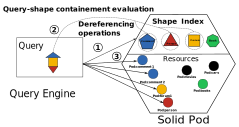
\includegraphics[width=0.51\textwidth]{figure/shape_containement}
    \caption{First, the shape index is dereferenced, 
    then the \emph{query-shape containment} operations are performed in the query engine and lastly, only the relevant resources are dereferenced.}
    \label{fig:shape_index}
\end{figure}

\section{Preliminary results}


\sepfootnotecontent{impl}{ The algorithm implementation is available at the following link \newline
\href{https://github.com/constraintAutomaton/query-shape-detection}{https://github.com/constraintAutomaton/query-shape-detection}
and the integration in the Comunica query engine at the following link 
\href{https://github.com/constraintAutomaton/comunica-feature-link-traversal/tree/feature/shapeIndex}{https://github.com/constraintAutomaton/comunica-feature-link-traversal/tree/feature/shapeIndex}.
The implementation of the benchmark and complementary results (such as the analysis of the statistical significance) are available at the following link 
\href{https://github.com/constraintAutomaton/amw_shape_index_results}{https://github.com/constraintAutomaton/amw\_shape\_index\_results}.
}


An open-source implementation of the \href{https://github.com/constraintAutomaton/query-shape-detection}{algorithm} and an 
\href{https://github.com/constraintAutomaton/comunica-feature-link-traversal/tree/feature/shapeIndex}{integration} in the query engine 
Comunica \cite{taelman_iswc_resources_comunica_2018} is available online~\sepfootnote{impl}.
We use the \href{https://github.com/SolidBench/SolidBench.js}{benchmark Solidbench} \cite{Taelman2023} to compare our approach with the current state-of-the-art (the \href{https://solid.github.io/type-indexes/}{type index} and the \href{https://www.w3.org/TR/ldp/}{LDP specification} as structural assumptions) \cite{Taelman2023}.
We used the supported subset of SolidBench queries, skipping the currently unimplemented \href{https://www.w3.org/TR/sparql11-query/#propertypaths}{SPARQL property paths} and nested queries.
We executed each query 50 times with a timeout of 1 minute (6,000 ms).
Figure \ref{fig:result} shows that the reduction can be as high as 80\% (D1V3 and S1V3) for execution time 
and 97\% (S1V3) for the number of HTTP requests.
Our approach reliably executes fewer HTTP requests compared to the state-of-the-art.
This is an expected result because no queries target (implicitly) each file of a user and the shape index approach requests a subset of the request of the type index approach (without sacrificing query results) with the addition of the request to get the shape definitions (which lead in general to the dereferencing of a small number of short documents).
There is not a direct correlation between the reduction of execution time and HTTP requests (e.g., the ratio 
between our approach and the state-of-the-art of the number of HTTP requests by the execution time for D1V3 is 0.5 compared to 0.15 for S1V3).
This hints at the results from the state-of-the-art \cite{Taelman2023} proposing that the query plan is the bottleneck for some queries in this environment,
however, the overhead of the containment calculation could also be a contributing factor to the current results.
In the worst cases, our approach  has similar query execution to the state-of-the-art (except for D3V3 and D3V4 with an increase of 9\% of the mean of the execution time).
Furthermore, their variances tend to be lower compared to their counterpart. 
One possible explanation for this observation is that the execution time of HTTP requests is unpredictable \cite{hartig2016walking}
leading to an increase in variance.
This observation not only has potential implications for the reliability of multiple executions in terms of execution time
but also in terms of the performance of single executions in unstable networks where the server might take longer times to respond. 

\begin{figure}
  \centering
  \includegraphics[width=0.93\linewidth]{figure/combined}
  \caption{
  The execution time with shape indexes is consistently lower (up to 80\% with D1V3 and S1V3) or equal to with the type indexes (except for D3V3 and D3V4), and always uses fewer HTTP requests.
  }
  \label{fig:result}
\end{figure}
\input{section/Conclusion}

% --- Bibliography ---

\bibliography{references}

\end{document}

%%
%% End of file
